\documentclass[USenglish,pdftex,compress,10pt,svgnamesi,handout]{beamer}
%\documentclass[USenglish,pdftex,compress,10pt,svgnames]{beamer}
\usepackage{import}\subimport{../../common/}{lectureheader}

\graphicspath{{pics/}}

\parskip2ex

\def\Vec#1{\textbf{#1}}
\newcommand{\scalar}[2]{#1^T#2}
\newcommand{\scalarold}[2]{\left<#1,#2\right>}




% =====================================================================
% Titel etc.
\hypersetup{%
	pdftitle={Optimisation in neural networks},%
	pdfauthor={Patrick van der Smagt}%
}

\title{optimisation in neural networks}
\author{Patrick van der Smagt}
\date{}
% =====================================================================
\begin{document}


%'''''''''''''''''''''''''''''''''''''''''''''''''''''''''
\begin{frame}
	\titlepage
	
	\vfil
\end{frame}


\begin{frame}
\frametitle{What is optimisation?}
We have a model $p_{\Vec w}(z\mid x)$.  This can, e.g., be a neural network.

We want to minimise the loss
$$
    \mathcal{L}(\Vec w) = -\log \prod_i p_{\Vec w}(z_i \mid x_i)
$$
by finding better values of $\Vec w$.

\end{frame}

\begin{frame}
\frametitle{How do we do optimisation?}
\begin{itemize}
\item if finding the best $\Vec w$ is a convex problem, good methods exist \\(remember SVD from linear algebra).

\item In general, finding the best $\Vec w$ is not a convex problem.  \\Only incremental methods are known.
\end{itemize}
\begin{columns}
\column{5cm}
\includegraphics[width=4cm]{convex}
\column{5cm}
\includegraphics[width=4cm]{nonvex}
\end{columns}

\end{frame}



\begin{frame}
\frametitle{Convex optimisation problems}
Practical example: $\{(x_i, z_i)\} = \{ (0,1); (1, 2.1); (2, 2.9)\}$.

Our model: $y_{\Vec w}(x) = a x + b$ with $\Vec w=(a,b)$; the MLE loss is
$$
\mathcal L(\Vec w) = \sum_i \bigl(y_{\Vec w}(x_i) - z_i\bigr)^2
$$

How do we find the minimum of $\mathcal L$?
  It is there where $\partial \mathcal L / \partial w_i = 0$.
  
  \pause 
  
  $$
{\partial \mathcal L_i(\Vec w) \over \partial w_1\equiv a} = 2 x_i (b + a x_i - z_i) = 0
$$
$$
{\partial \mathcal L_i(\Vec w) \over \partial w_2\equiv b} = 2 (b + a x_i - z_i) = 0 
$$

We can solve that!
\end{frame}
   \begin{frame}
\includegraphics[width=\textwidth]{simpleefunc}

Numerical solution: $a=0.95, b=1.05$.
\end{frame}

% =====================

\begin{frame}
\frametitle{What if\dots}
$y_{(a,b,c)}(x) = {\color{red}a} \exp(-{\color{red}b}(\Vec x-{\color{red}c})^2) + d$

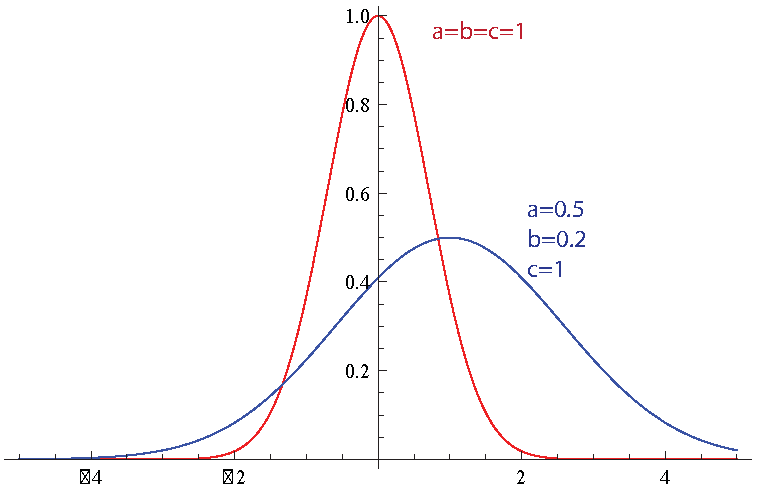
\includegraphics[width=8cm]{pics/exp}

We can't find a closed-form solution for that!
\end{frame}

\begin{frame}
\begin{align*}
2 e^{-b c^2} \left(a e^{-b c^2}-1\right)+2 e^{-b (1-c)^2} \left(a e^{-b (1-c)^2}-2.1\right)+&\\
2 e^{-b (2-c)^2}
   \left(a e^{-b (2-c)^2}-2.9\right)&=0
   \end{align*}
   
 \begin{align*}
-2 a c^2 e^{-b c^2} \left(a e^{-b c^2}-1\right)-2 a (1-c)^2 e^{-b (1-c)^2} \left(a e^{-b (1-c)^2}-2.1\right)-&\\
2   a (2-c)^2 e^{-b (2-c)^2} \left(a e^{-b (2-c)^2}-2.9\right)&=0
   \end{align*}
   
 \begin{align*}
-4 a b c e^{-b c^2} \left(a e^{-b c^2}-1\right)+4 a b (1-c) e^{-b (1-c)^2} \left(a e^{-b (1-c)^2}-2.1\right)+&\\
4
   a b (2-c) e^{-b (2-c)^2} \left(a e^{-b (2-c)^2}-2.9\right)&=0
   \end{align*}
\end{frame}
   \begin{frame}
\includegraphics[width=\textwidth]{weirdfunc}

$c = -1$
\end{frame}

   

\begin{frame}
\frametitle{But}
We can compute $\partial \mathcal L(\Vec w) / \partial w_i$
\end{frame}




\begin{frame}
\frametitle{the value of $\mathcal L$}
we are interested in finding $\argmin_{\Vec w} \mathcal L$

\includegraphics[width=8cm]{pics/optimise1.png}

\end{frame}


\begin{frame}
\frametitle{using local information $\mathcal L(\Vec w)$}
we are interested in finding $\argmin_{\Vec w} \mathcal L$ 


\includegraphics[width=8cm]{pics/optimise2l.png}
\end{frame}


\begin{frame}
\frametitle{using local information $\mathcal L(\Vec w)$ as well as $\partial \mathcal L(\Vec w)/\partial w$}
we are interested in finding $\argmin_{\Vec w} \mathcal L$ 


\includegraphics[width=8cm]{pics/optimise2.png}

\end{frame}


\begin{frame}
\frametitle{using the gradient $\Vec g$ of $\mathcal L$}

\begin{columns}
\begin{column}{5cm}
The direction $\Vec u$ in which to optimise is given by the gradient: $\Vec u = -\Vec g$
\end{column}
\begin{column}{5cm}
\centerline{\includegraphics[width=5cm]{pics/optimise5.png}}
\end{column}
\end{columns}
Searching the minimum by repeated evaluation of $\mathcal L$ and $\Vec g \equiv \nabla \mathcal L$. \\
$-\Vec g$ 
gives us a direction $\Vec u$  in which we want to optimise.  \\
We change the parameter vector as follows:
\begin{align}
\Vec u_i &= -\Vec g_i \\
\Vec w_{i+1} &= \Vec w_i +  \alpha \Vec u_i 
\end{align}
we call $\Vec u$ the \alert{search direction}\\
we call $\alpha$ the \alert{learning parameter} or \alert{step size}\\
we call this method \alert{steepest descent} or \alert{gradient descent}\\
it belongs to the class of {greedy algorithms}
\end{frame}



\begin{frame}
\frametitle{the value of $\alpha$}

a \textsl{too small} value for $\alpha$ has two drawbacks:
\begin{itemize}
\item we find the minimum more slowly\pause
\item we end up in local minima or saddle/flat points
\end{itemize}

\centerline{\includegraphics[width=6cm]{pics/optimise6.png}}

\end{frame}



\begin{frame}
\frametitle{the value of $\alpha$}

a \textsl{too large} value for $\alpha$ has one drawback:
\begin{itemize}
\item you may never find a minimum; oscillations usually occur
\end{itemize}

\centerline{\includegraphics[width=6cm]{pics/optimise7.png}}

we only need 2 steps to overshoot!
\end{frame}




\begin{frame}
\frametitle{putting a trace on $\Vec u$}

\centerline{\includegraphics[width=8cm]{pics/momentum.pdf}}
a: $\Vec u = -\Vec g$; small $\alpha$;\\
b: $\Vec u = -\Vec g$; large $\alpha$;\\
c: \begin{eqnarray}
\Vec u_{0} &=& -\Vec g_{0}\\
\Vec u_{i} &=& -\Vec g_{i} + \beta\Vec u_{i-1}\\
		&=& -\Vec g_{i} - \beta\Vec g_{i-1}  - \beta^2\Vec g_{i-2}  - \beta^3\Vec g_{i-3} \dots\\
\Vec w_{i+1} &=& \Vec w_{i} + \alpha \Vec u_{i} 
\end{eqnarray}
we call $\alpha$ the \alert{learning rate}\\
we call $\beta$ the \alert{momentum}\\
we usually take $\beta \gg \alpha$


\end{frame}




\begin{frame}
\frametitle{trick: momentum}
How do we choose $\alpha$ and $\beta$? 
if, for the sake of the argument, assume that  $\Vec g\equiv\nabla E$ does not change:
\begin{eqnarray*}
\Delta\Vec w &=& - \alpha\,\Vec g \,(1 + \beta + \beta^2 + \ldots) \\
		&=& -{\alpha \over 1-\beta} \,\Vec g
\end{eqnarray*}
\pause
Assuming a perfect $\nabla E$, the best values for $\alpha$ and $\beta$ are when
$$
  {\alpha \over 1-\beta}=1 \qquad \Rightarrow \qquad \alpha+\beta=1
$$
Typically we choose $\alpha$ small and $\beta$ large (of course, $\alpha,\beta>0$).

\end{frame}





\begin{frame}
\frametitle{bird's eye view}
\includegraphics[height=35mm]{pics/xx.pdf} \quad\quad=\quad\quad
\includegraphics[height=35mm]{pics/H1.pdf}

\pause
$$
\mathcal L(x) = \mathcal L(0) + x \underbrace{\partial \mathcal L \over \partial w}_g 
		+ x^2\underbrace{\partial^2 \mathcal L \over \partial w^2}_{\textrm{Hessian} H}
$$
\end{frame}




\begin{frame}
\frametitle{optimising}
following the gradient is not always the best choice

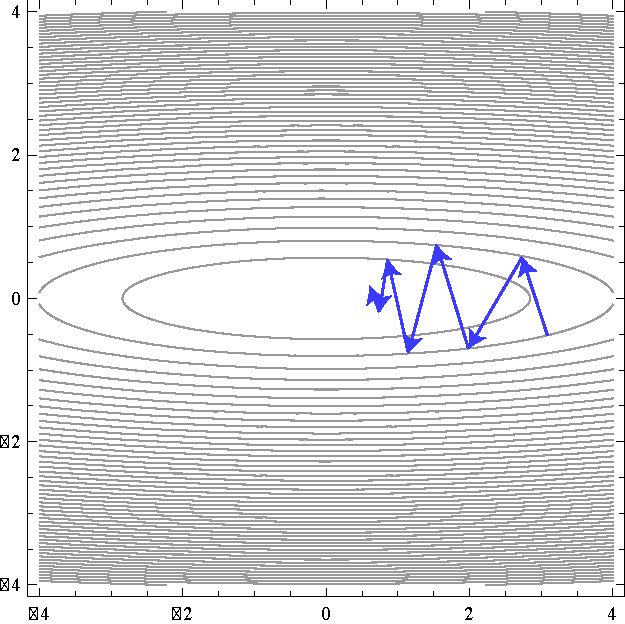
\includegraphics[height=60mm]{pics/H5opt.pdf}

Close to minima, it appears that Loss functions are close to quadratic
\end{frame}


\begin{frame}
\frametitle{condition of the Hessian}
Condition = largest EV / smallest EV

\bigskip

\begin{tabular}{cc}
Condition 5 & Condition 100\\
\includegraphics[height=40mm]{pics/H5.pdf}
&\includegraphics[height=40mm]{pics/H100.pdf}
\end{tabular}

What does $H$ look like?

A large condition number means that some directions of $H$ are very steep compared to others.
In neural networks, a condition of $10^{10}$ is not uncommon.

A class of optimisers (CG, Adam, rprop, adadelta, \dots) deal with such $H$.
\end{frame}


\begin{frame}
One resource I like in particular: \url{https://www.benfrederickson.com/numerical-optimization/}
\end{frame}
\end{document}






